\documentclass[12pt,aspectratio=169,notheorems]{beamer}
\graphicspath{
	{img/architecture}
	{img/db}
	{img/gachas/final}
	{img/logo-unipi}
}

\usetheme[progressbar=frametitle, numbering=fraction]{metropolis}
\usepackage{appendixnumberbeamer}
\usepackage[font=small,labelfont=bf]{caption}

\setbeamercolor{background canvas}{bg=white}

\usepackage{booktabs}
\usepackage[scale=2]{ccicons}

% Change Color of the theme
\usepackage{xcolor}
\definecolor{DarkGrey}{HTML}{353535}
\definecolor{ECNURed}{RGB}{164,31,53}
\definecolor{ECNUBrown}{RGB}{134,117,77}
\setbeamercolor{normal text}{ fg= DarkGrey  }
\setbeamercolor{alerted text}{ fg= ECNURed  }
\setbeamercolor{example text}{ fg= ECNUBrown  }

% Bolder Fonts for presenting in a large room 
\setsansfont[BoldFont={Fira Sans SemiBold}]{Fira Sans Book}

\title{\LARGE General architecture delivery}
\author{{\large \emph{EzGacha} \\[3ex]} Gioele Dimilta \\ Andrea Mugnai \\ Jacopo Tucci}
\date{}
\titlegraphic{\hfill
\includegraphics[height=1.8cm]{logo.png}}

\begin{document}

\maketitle

\begin{frame}{Player representation}
    A player is represented only by his \textbf{account} and there is no profile customization available. A player's account is based on the following data.
    \begin{itemize}
        \item Username
        \item Password
        \item Wallet (in-game currency)
    \end{itemize}
    Moreover, each player has some additional info related to the game.
    \begin{itemize}
        \item Gatcha collection
        \item Transactions history
    \end{itemize}
\end{frame}

\begin{frame}{Gachas}
    \vspace{3ex}
    \begin{columns}
        \begin{column}{.85\textwidth}
            \begin{tabular}{ccccc}
                    C & UC & R & E & S \\
                     
\includegraphics[width=.16\textwidth]{Skeleton mage (common).jpg} &
                     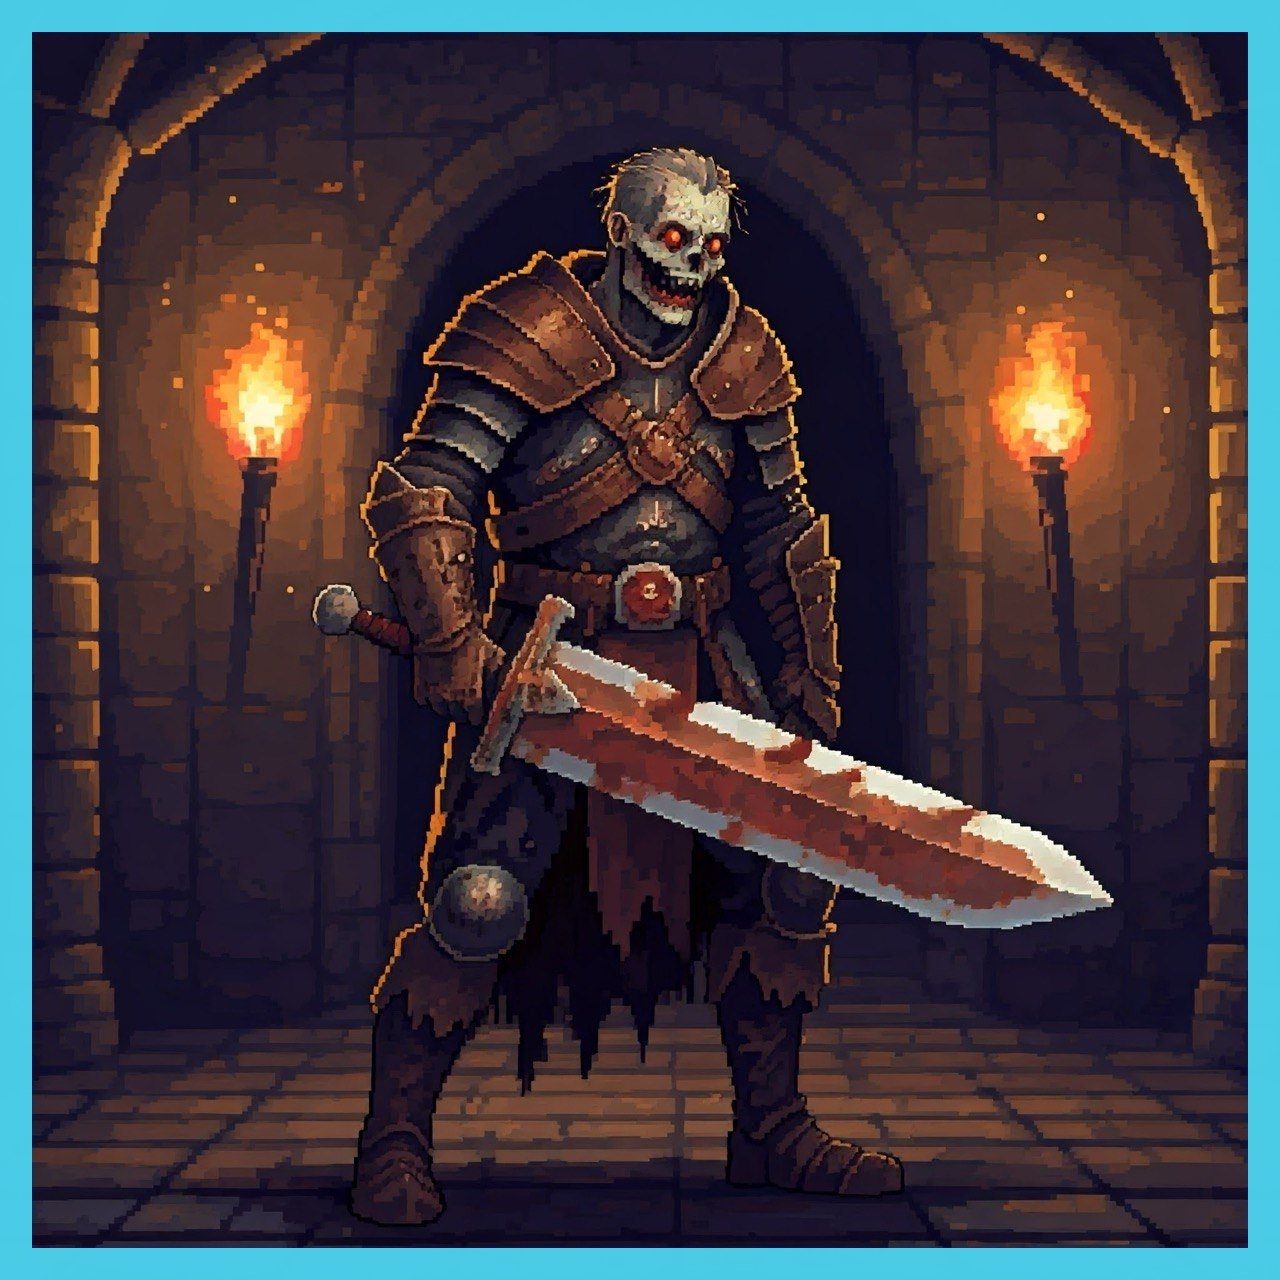
\includegraphics[width=.16\textwidth]{Undead (non-common).jpg} & 
                     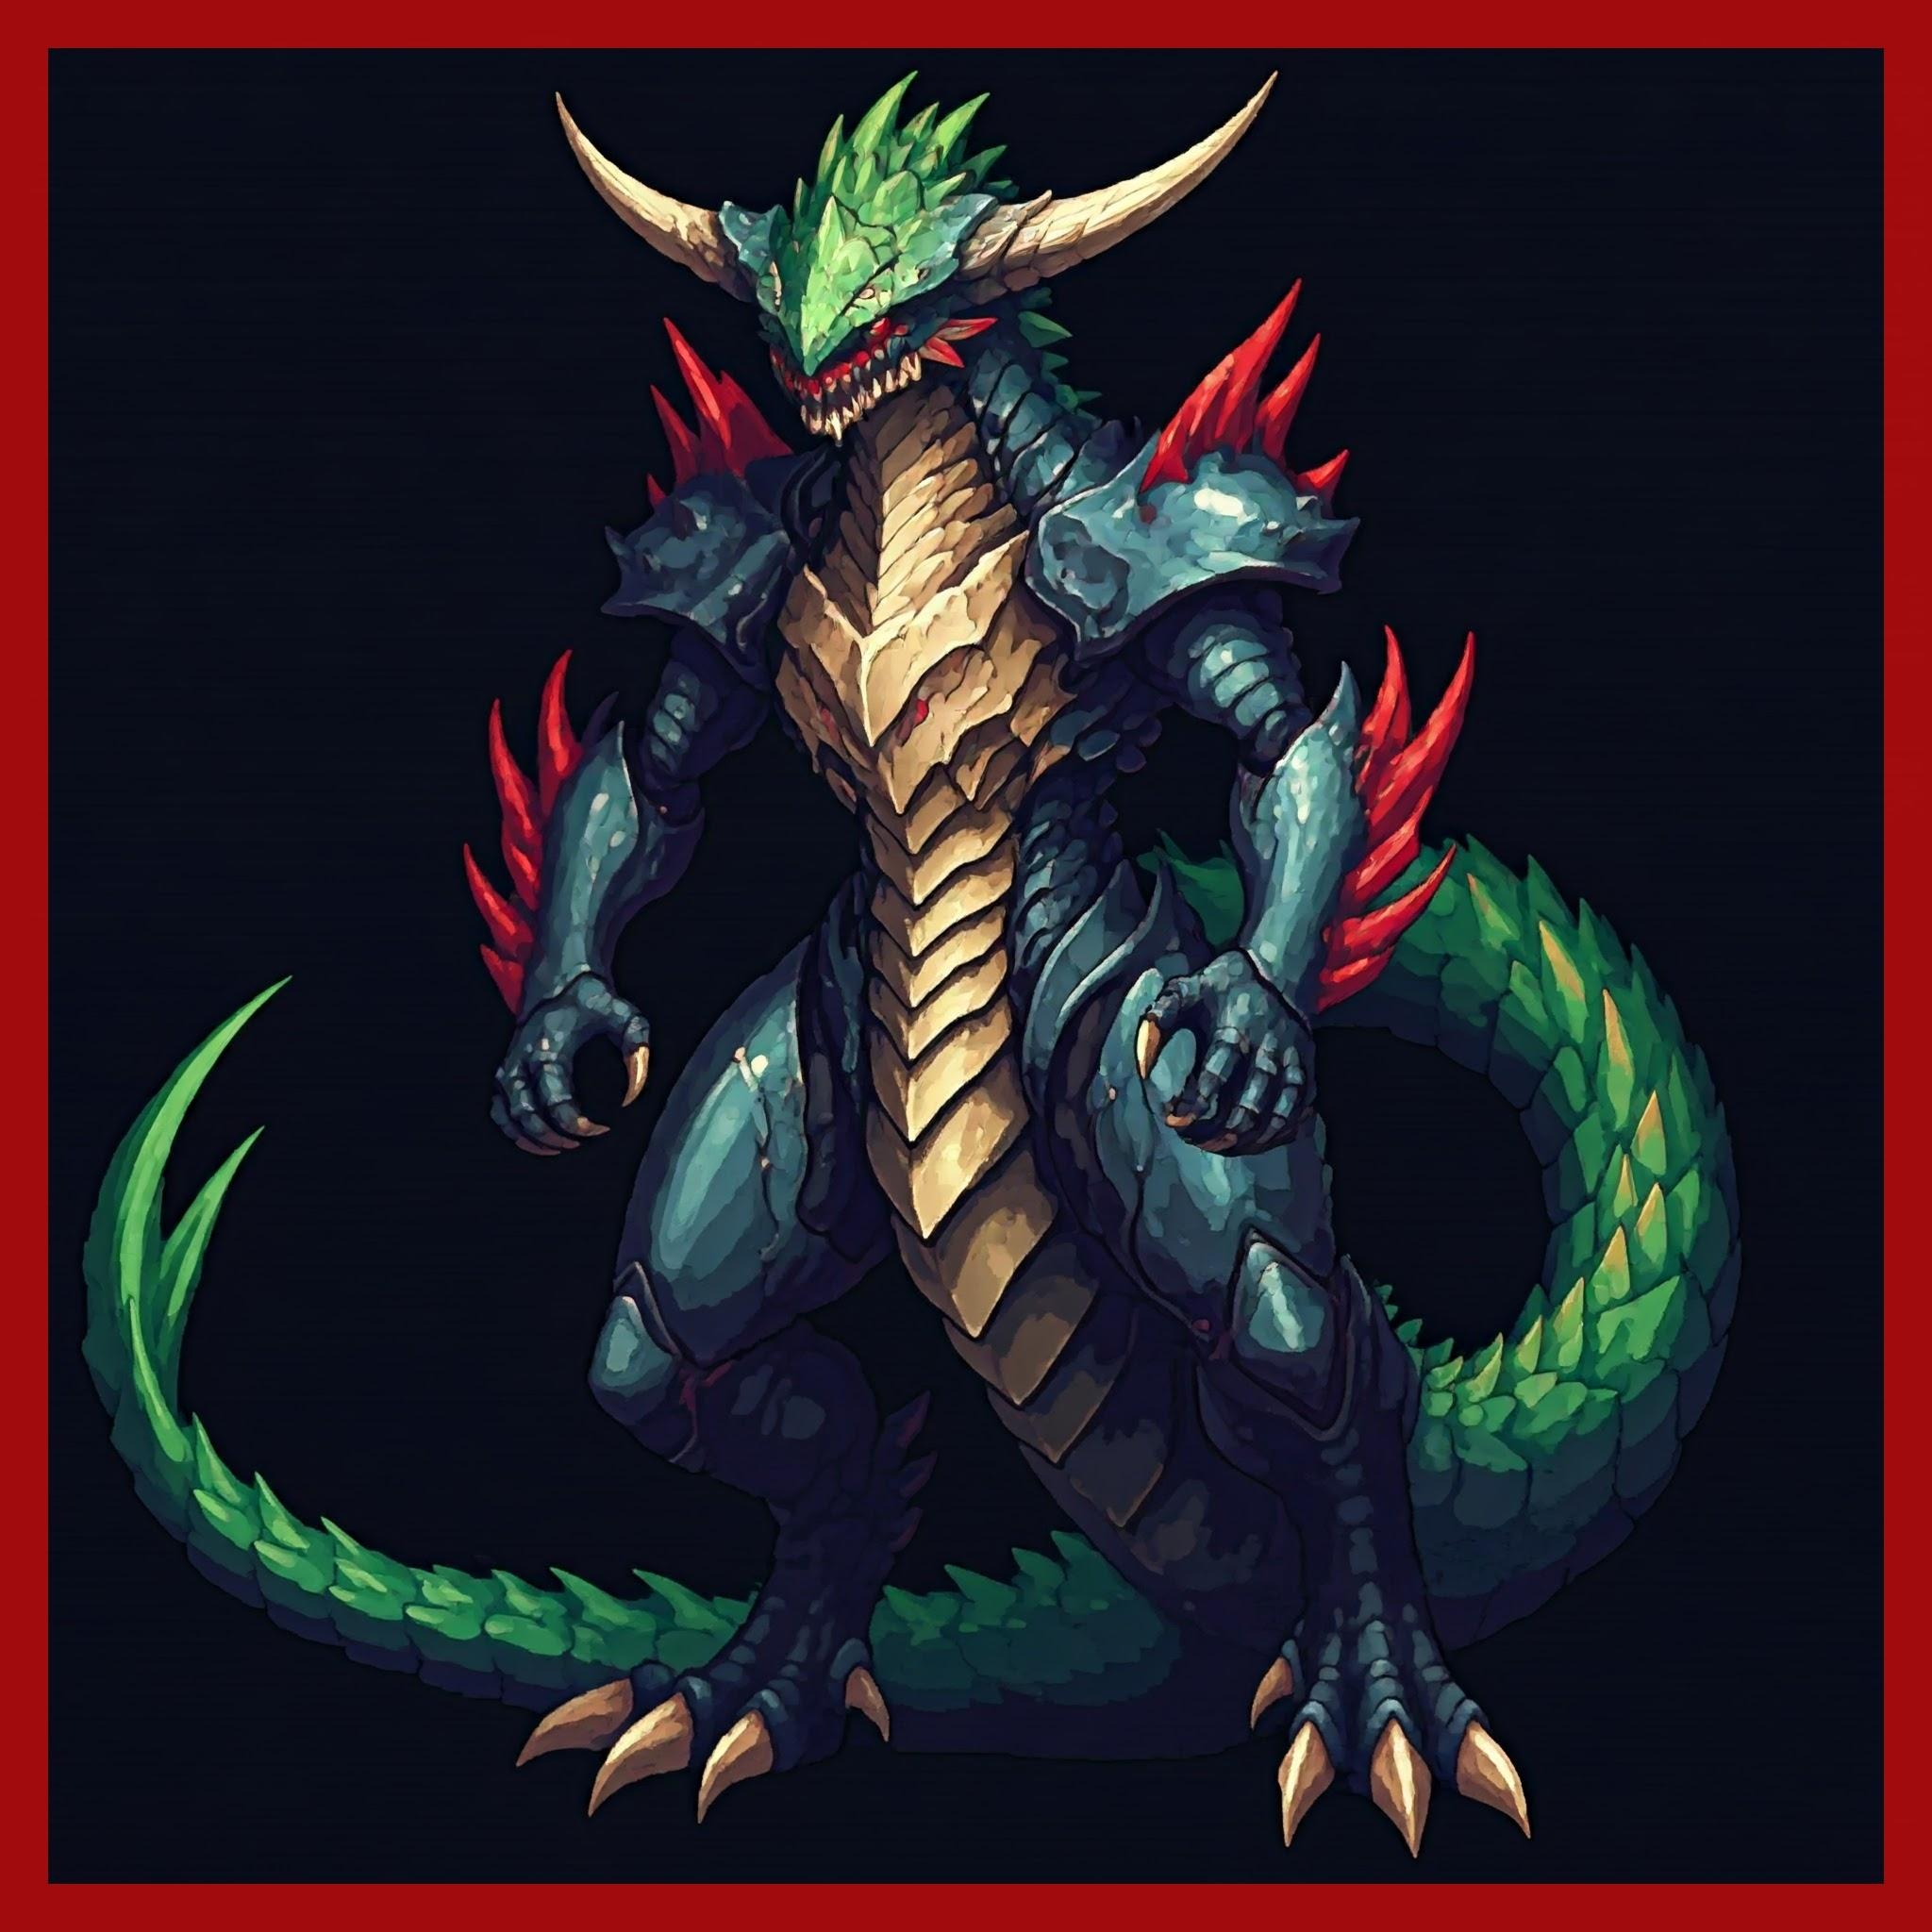
\includegraphics[width=.16\textwidth]{Demon (rare).jpg} &
                     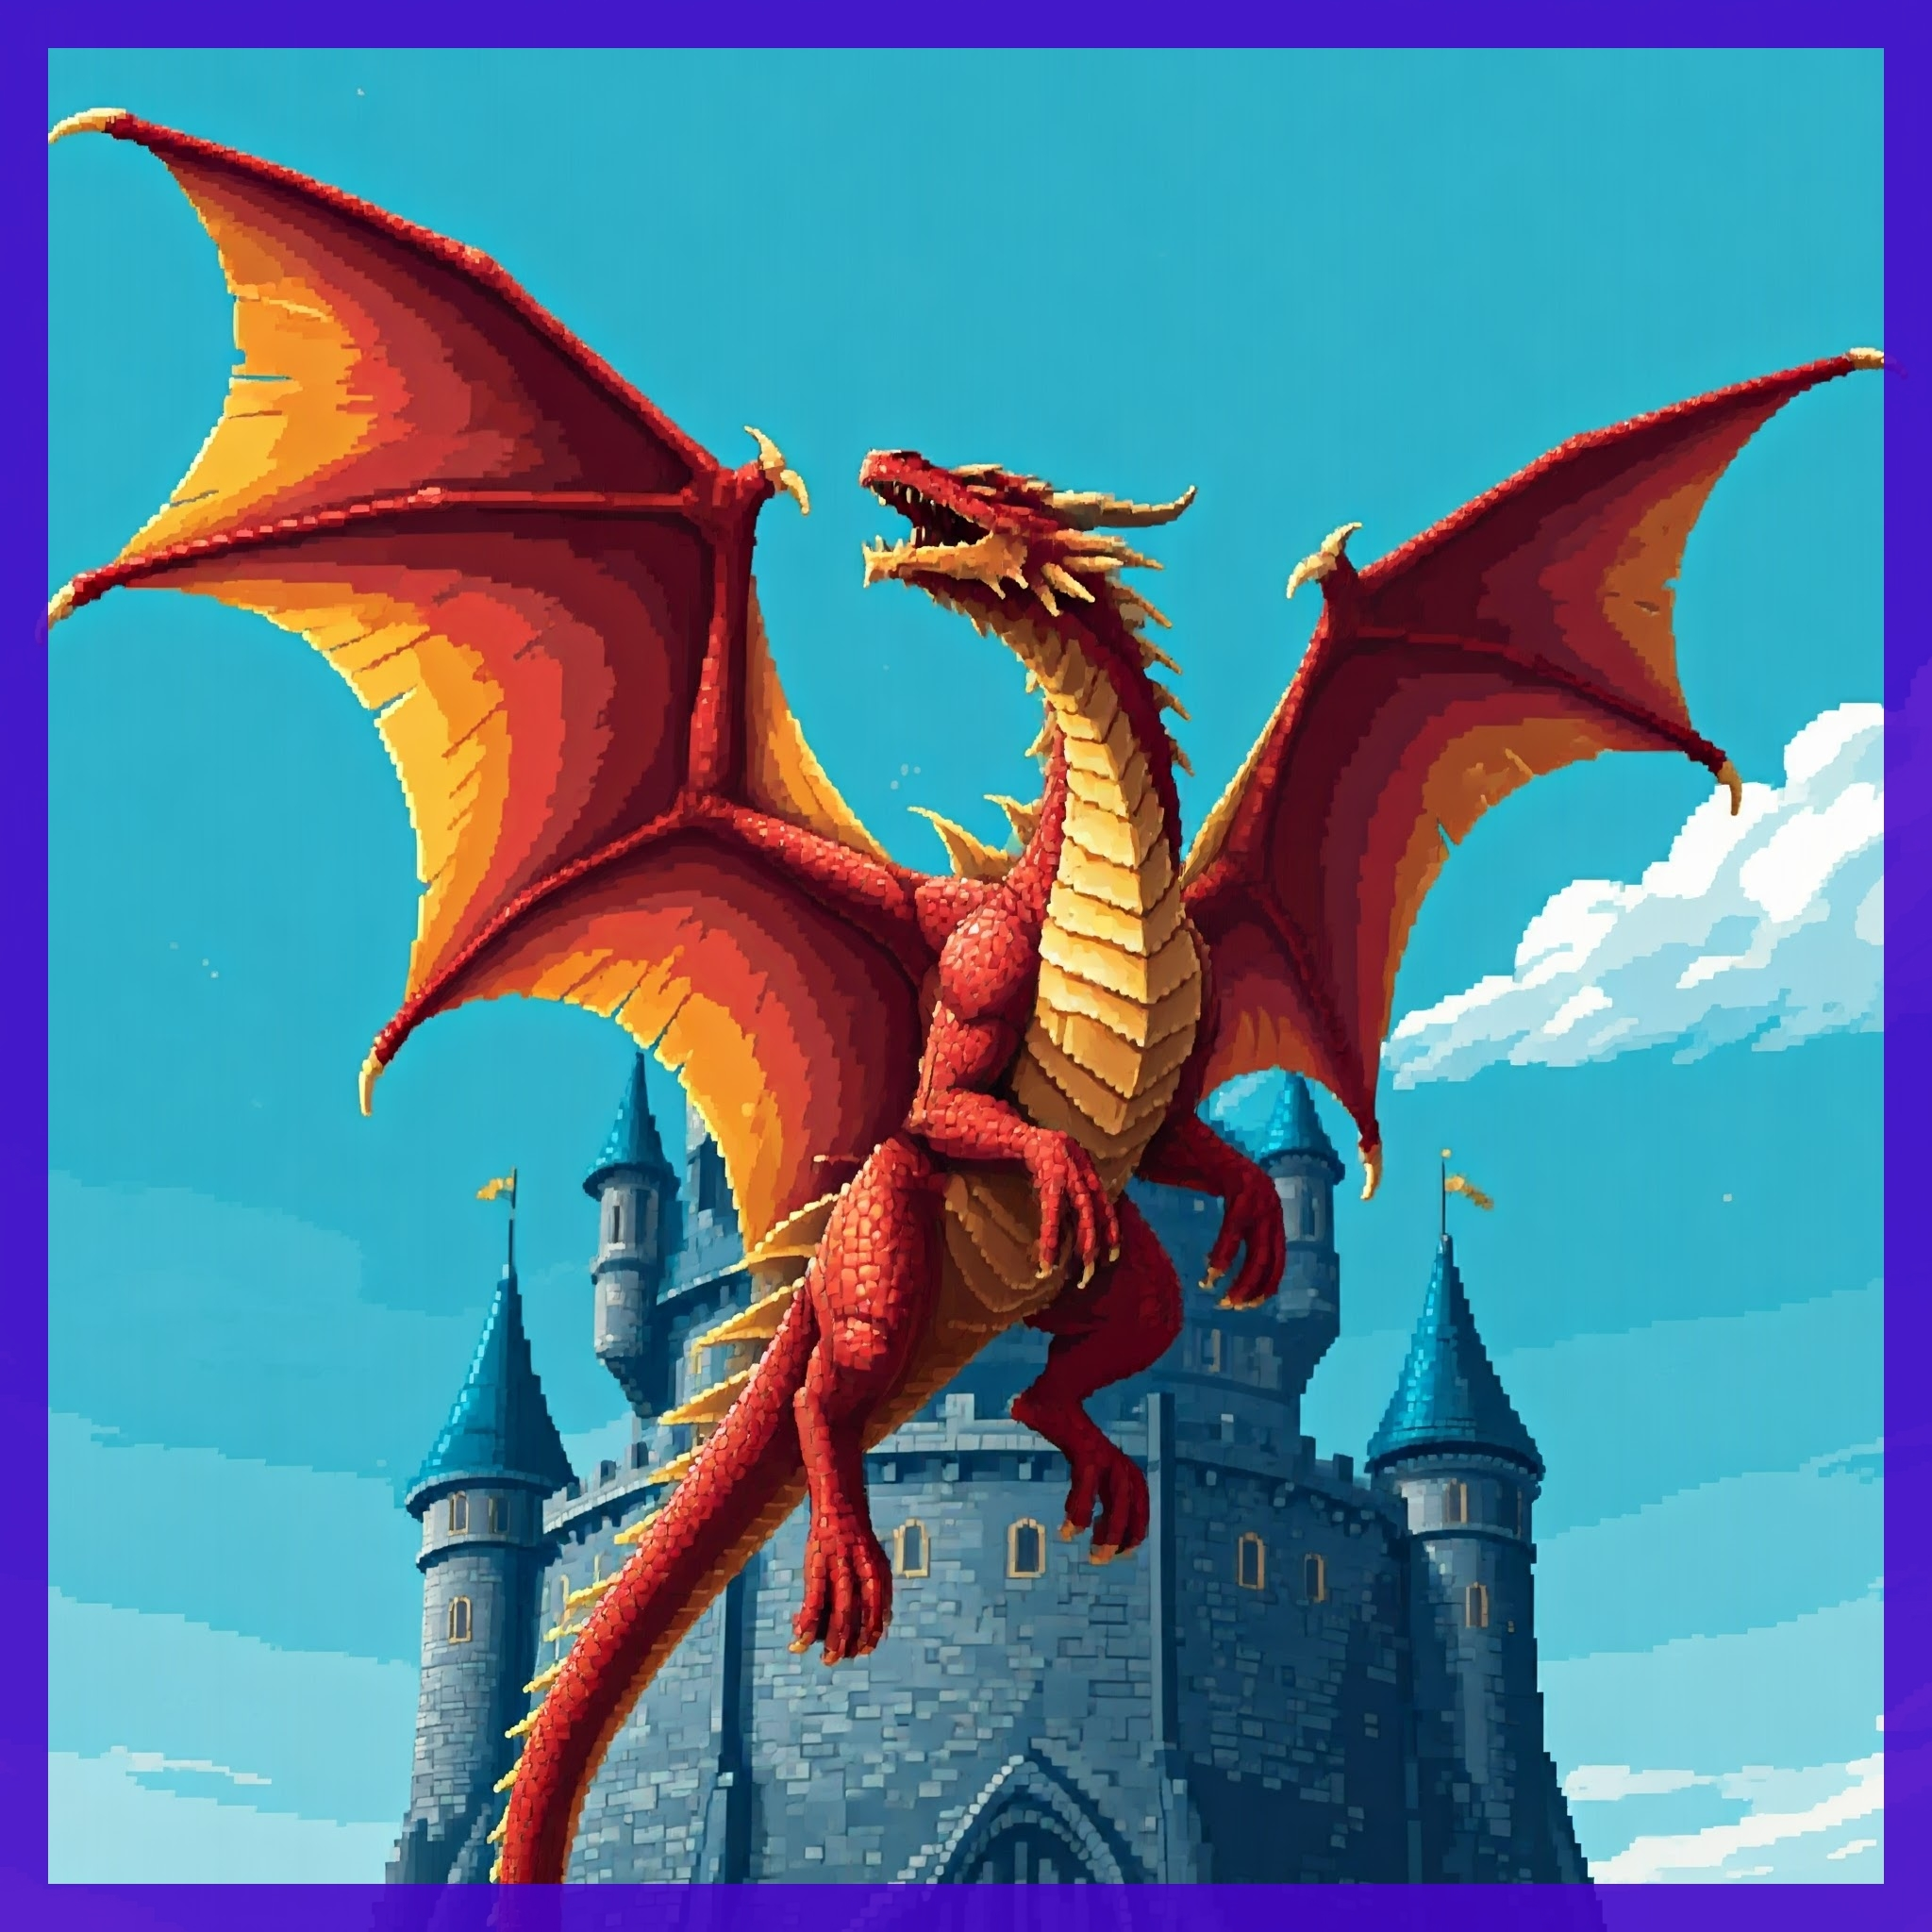
\includegraphics[width=.16\textwidth]{Dragon (epic).jpg} & 
                     
\includegraphics[width=.16\textwidth]{Phoenix (legendary).jpg} \\
                     
                    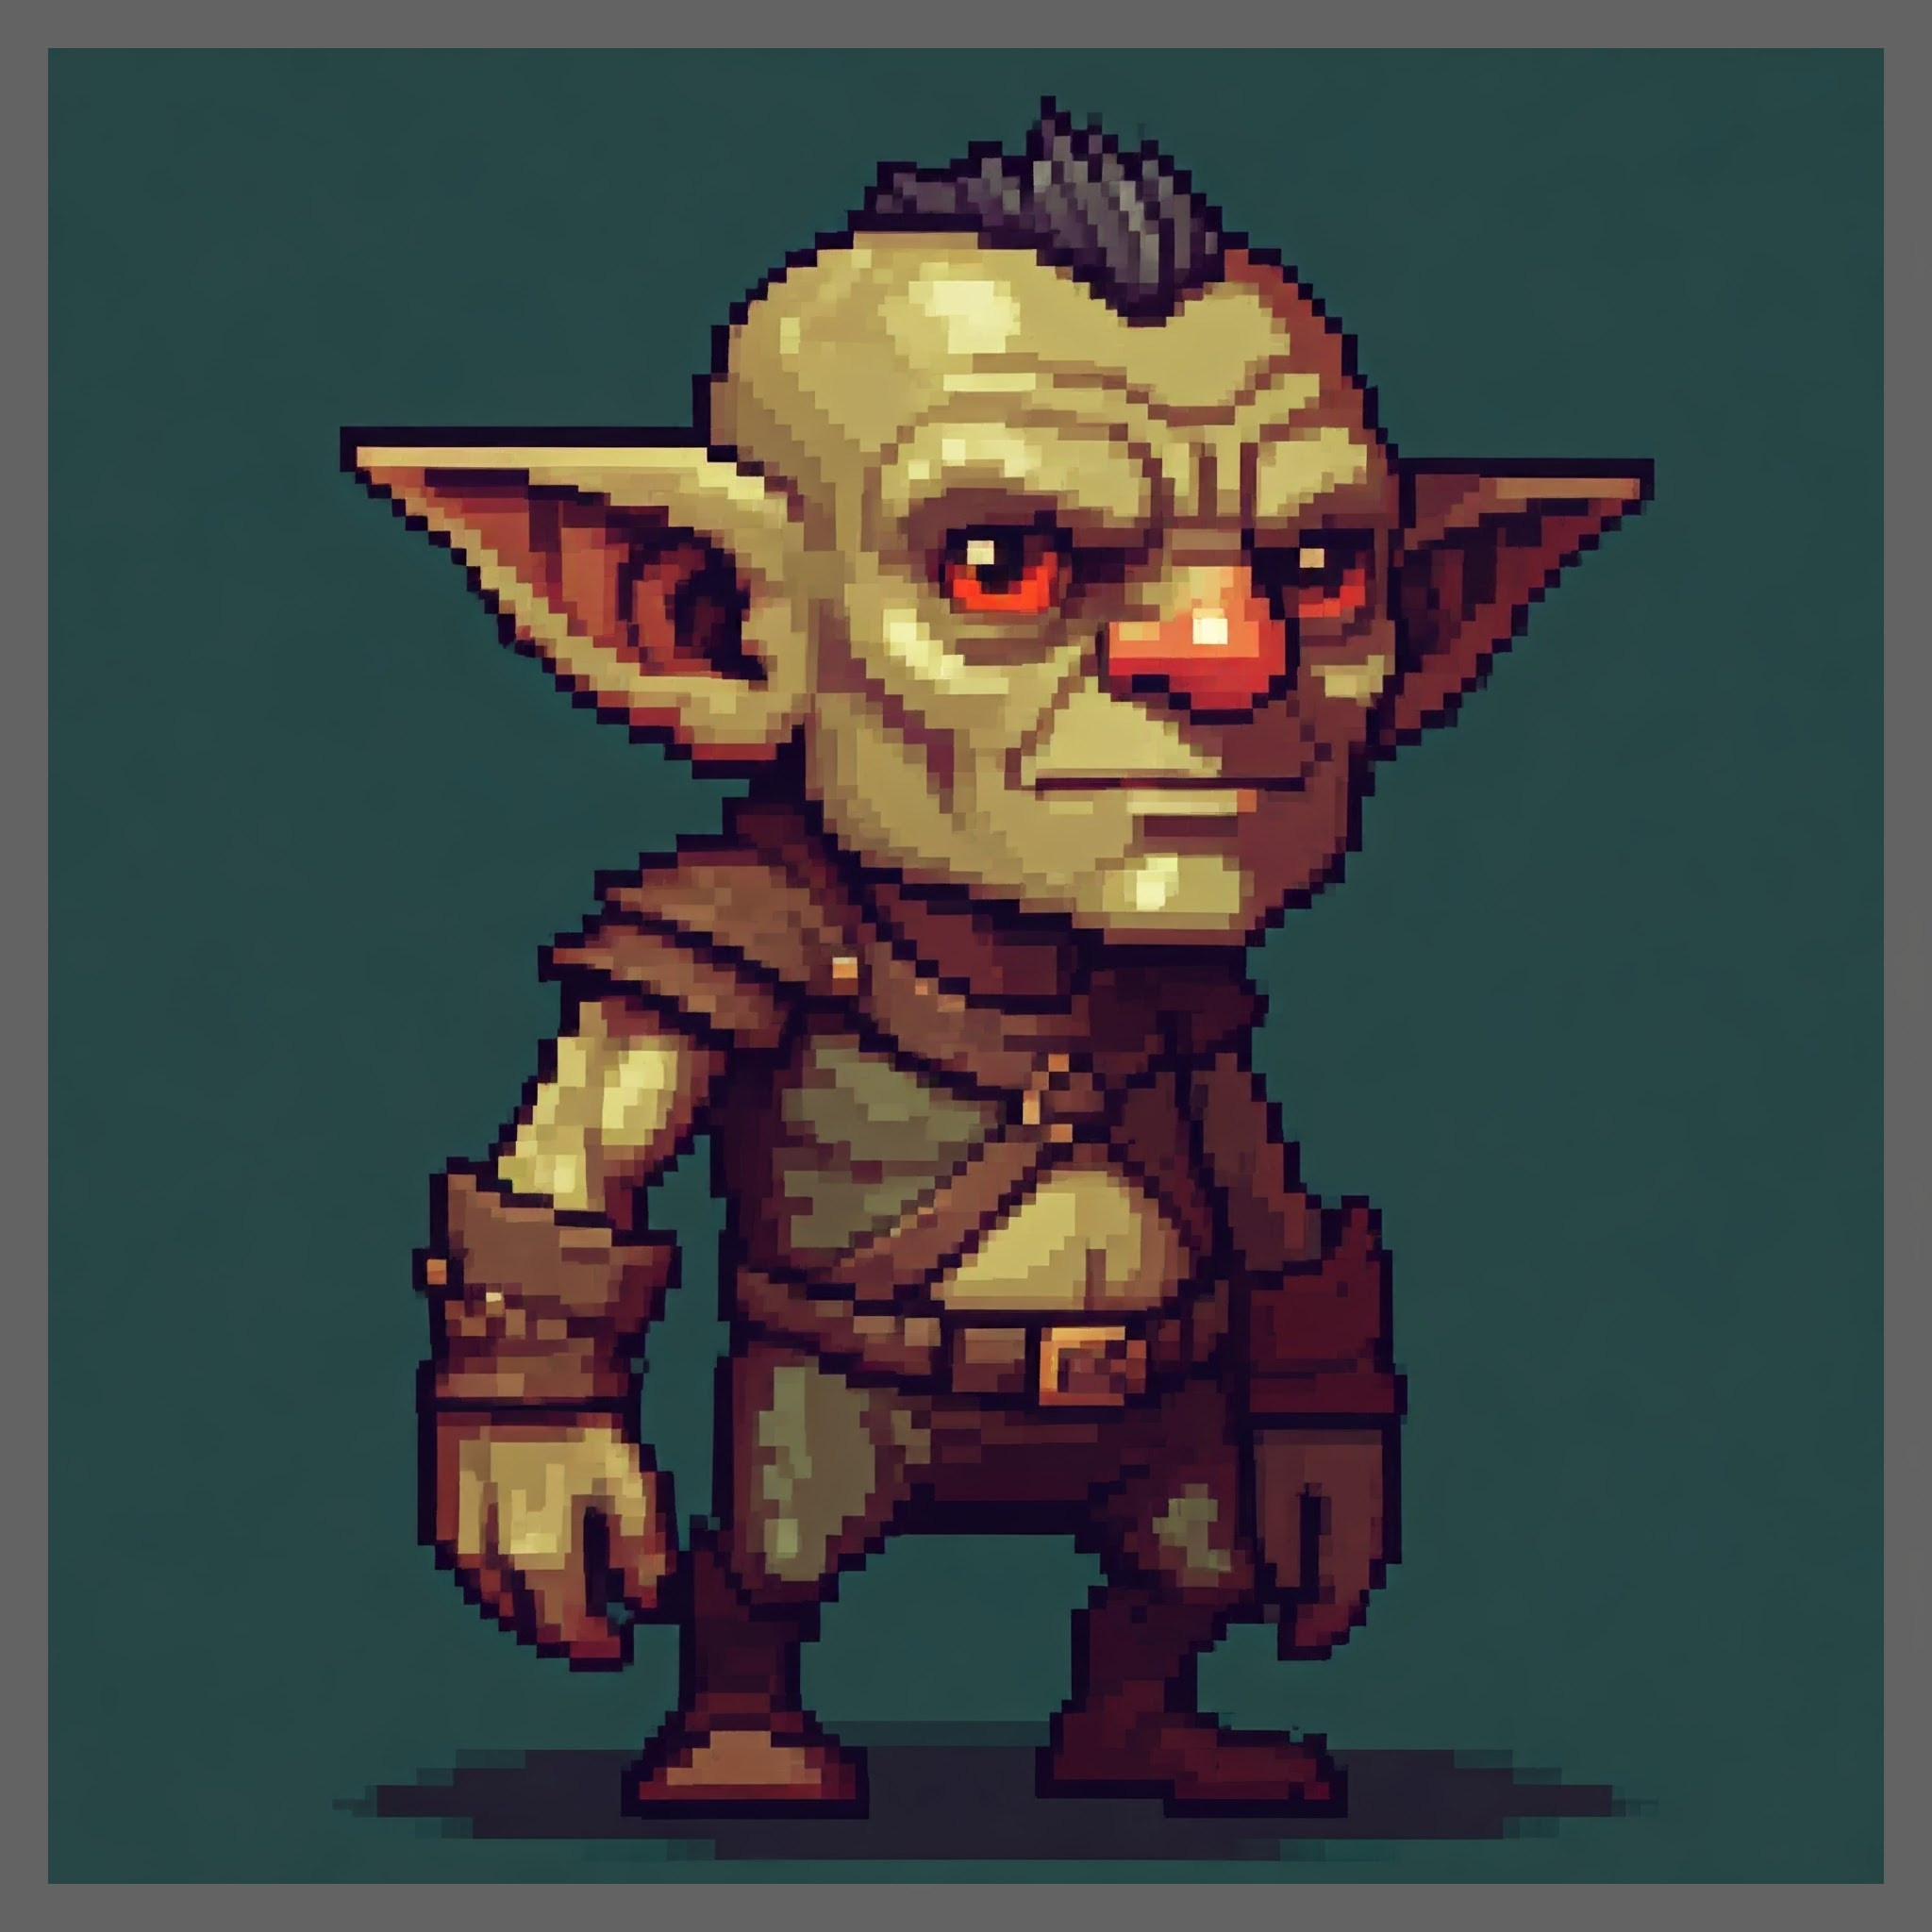
\includegraphics[width=.16\textwidth]{Goblin (common).jpg} &
                    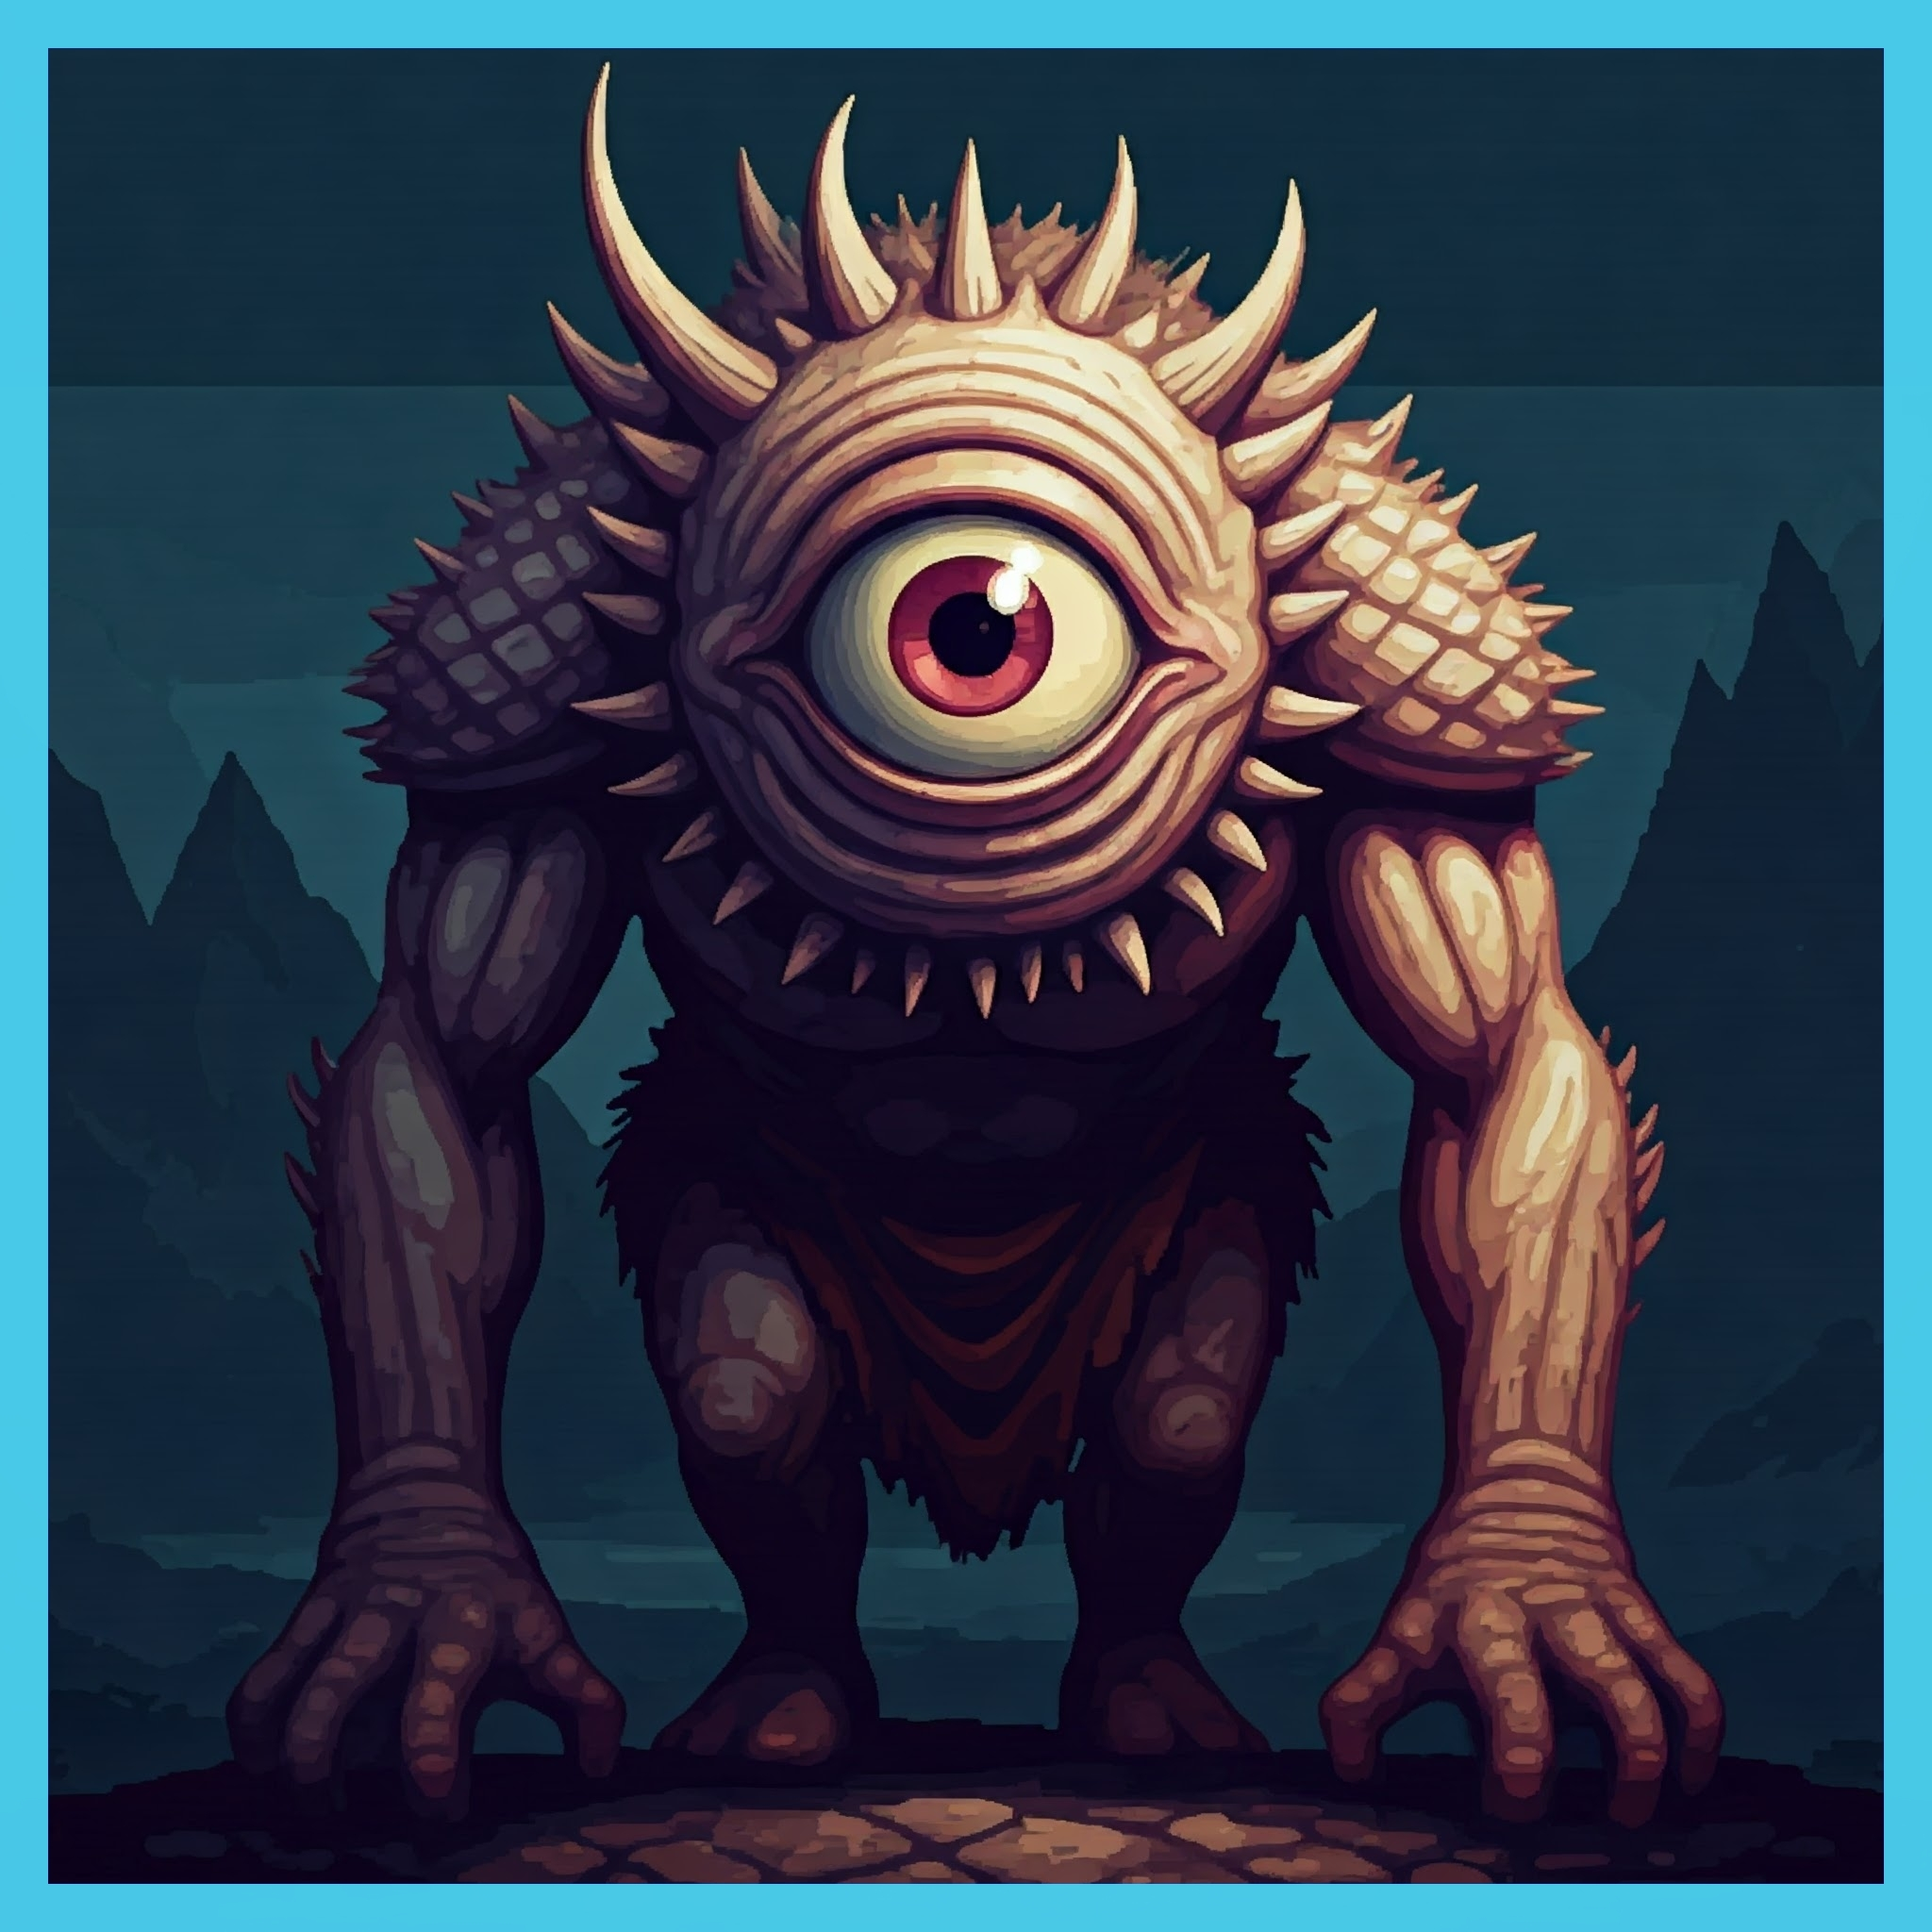
\includegraphics[width=.16\textwidth]{Cyclops (non-common).jpg} & 
                    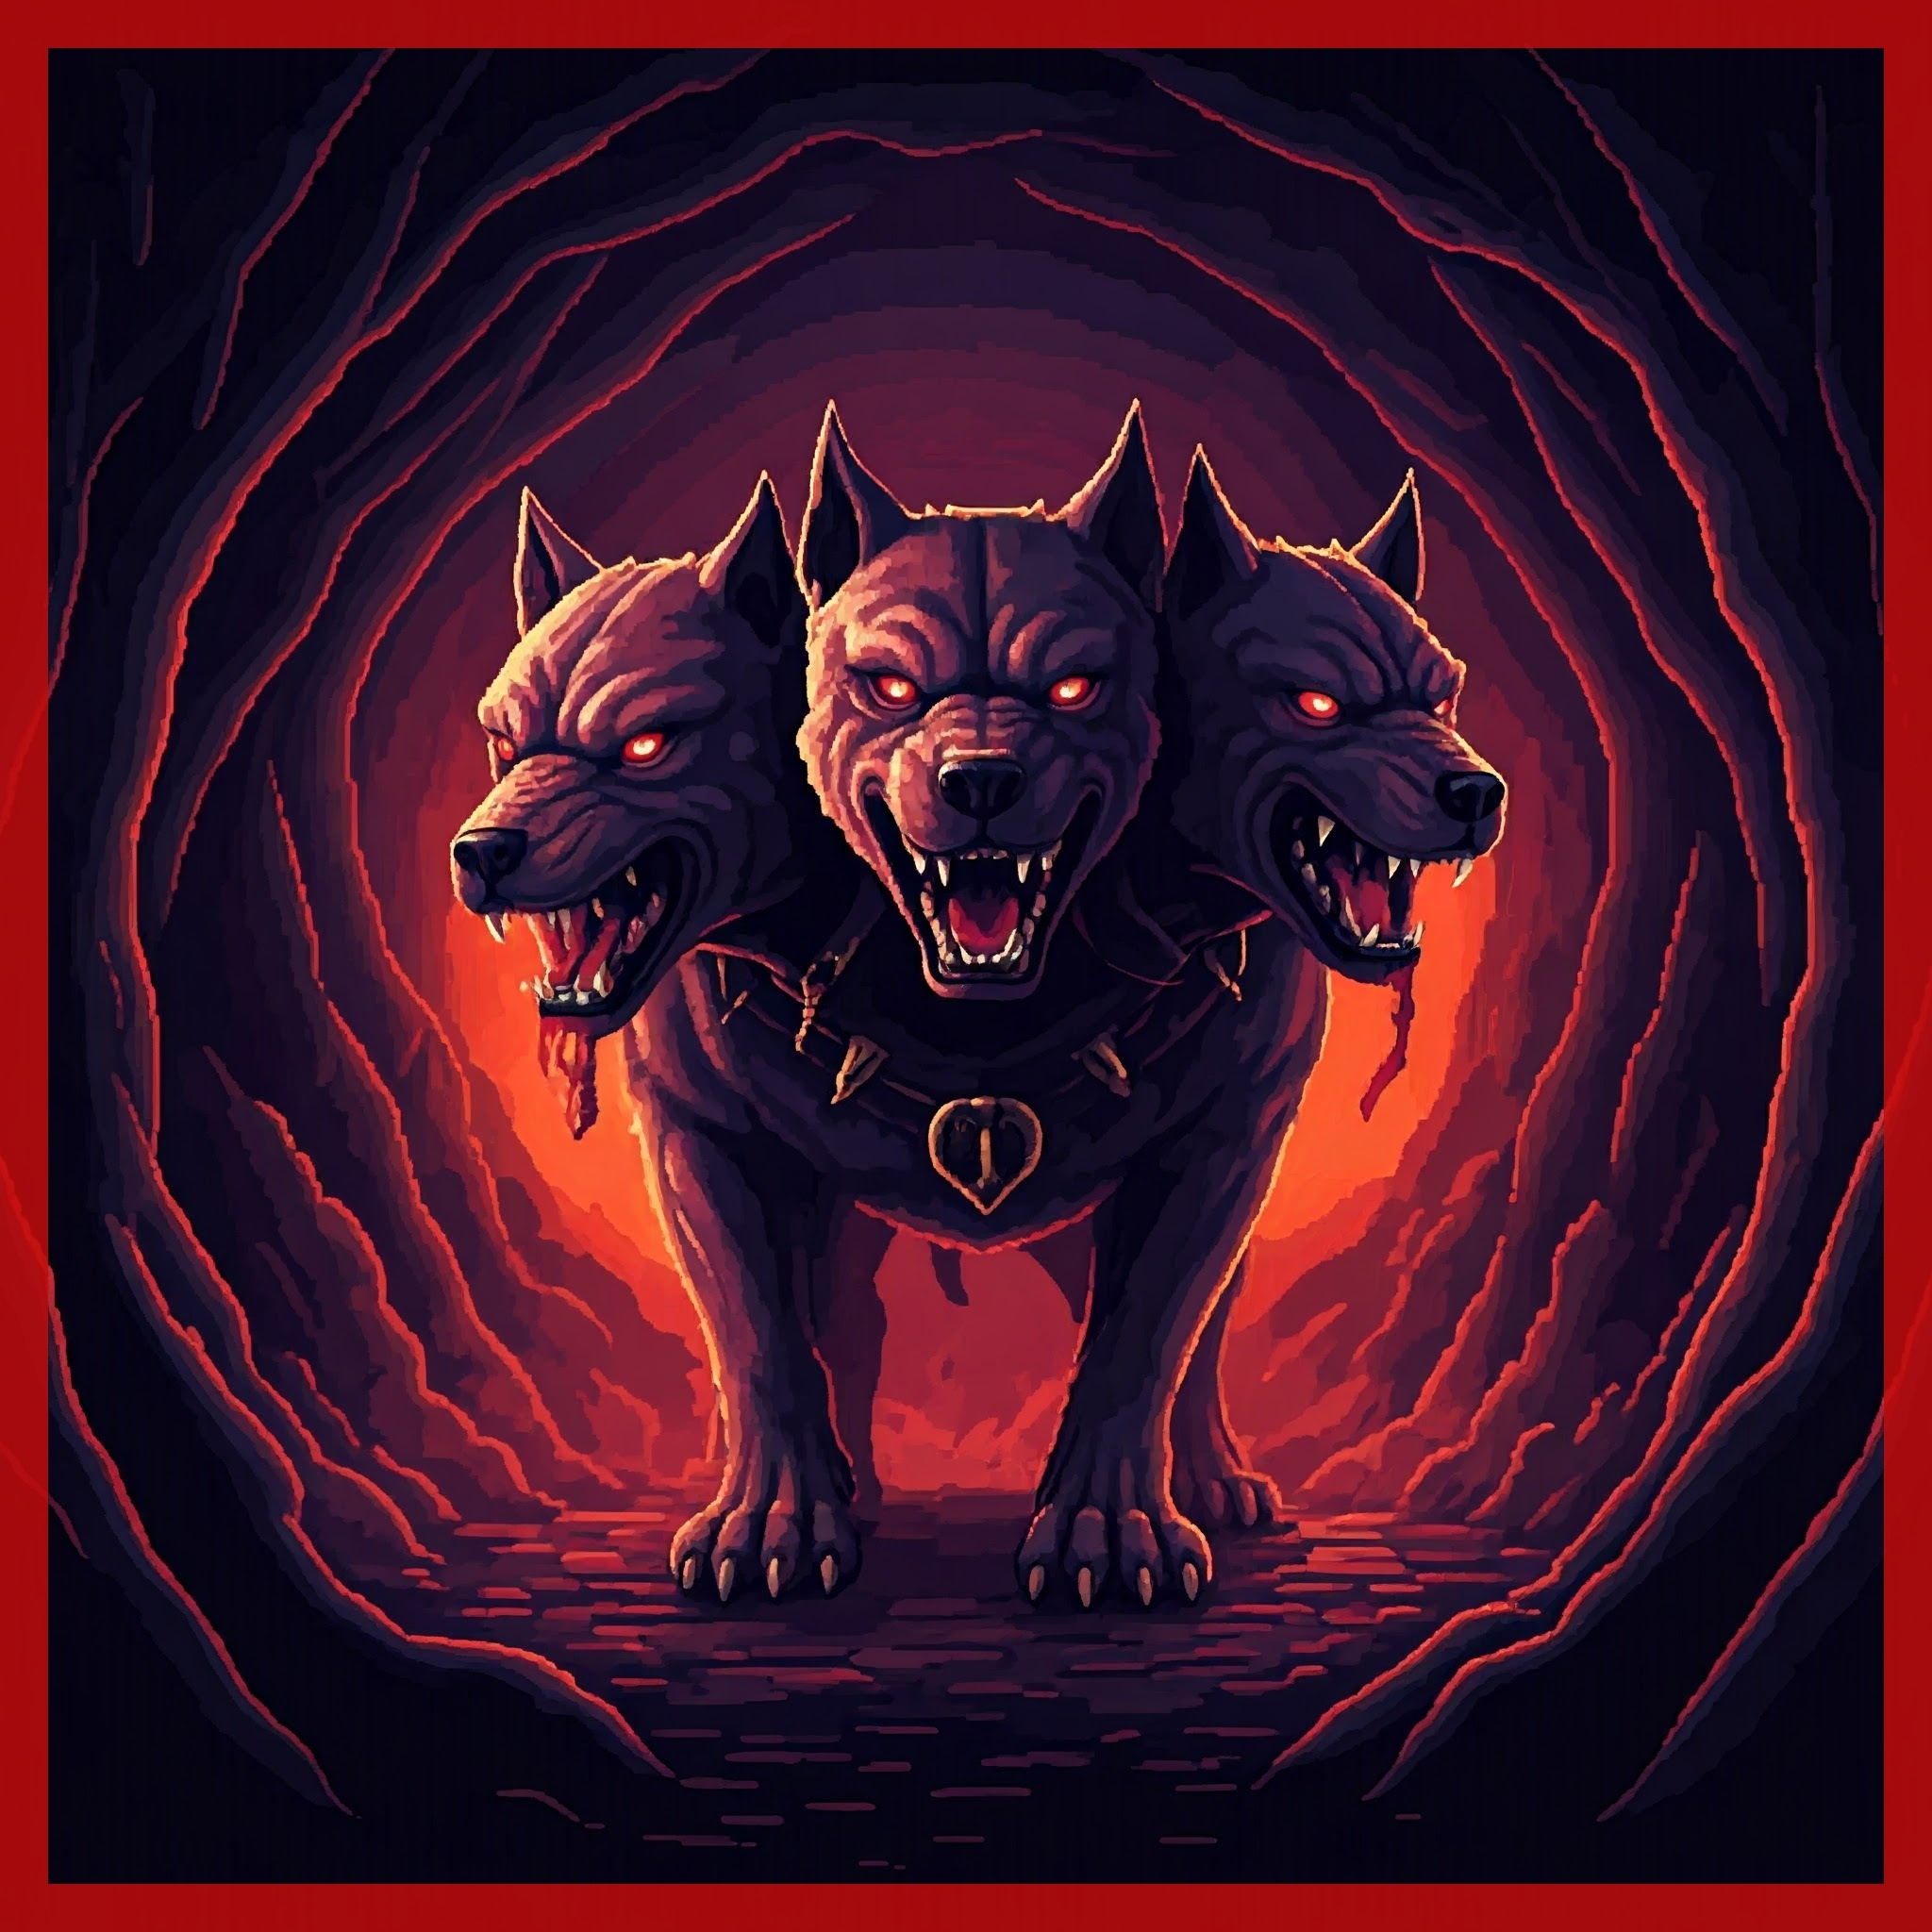
\includegraphics[width=.16\textwidth]{Cerberus (rare).jpg} &
                    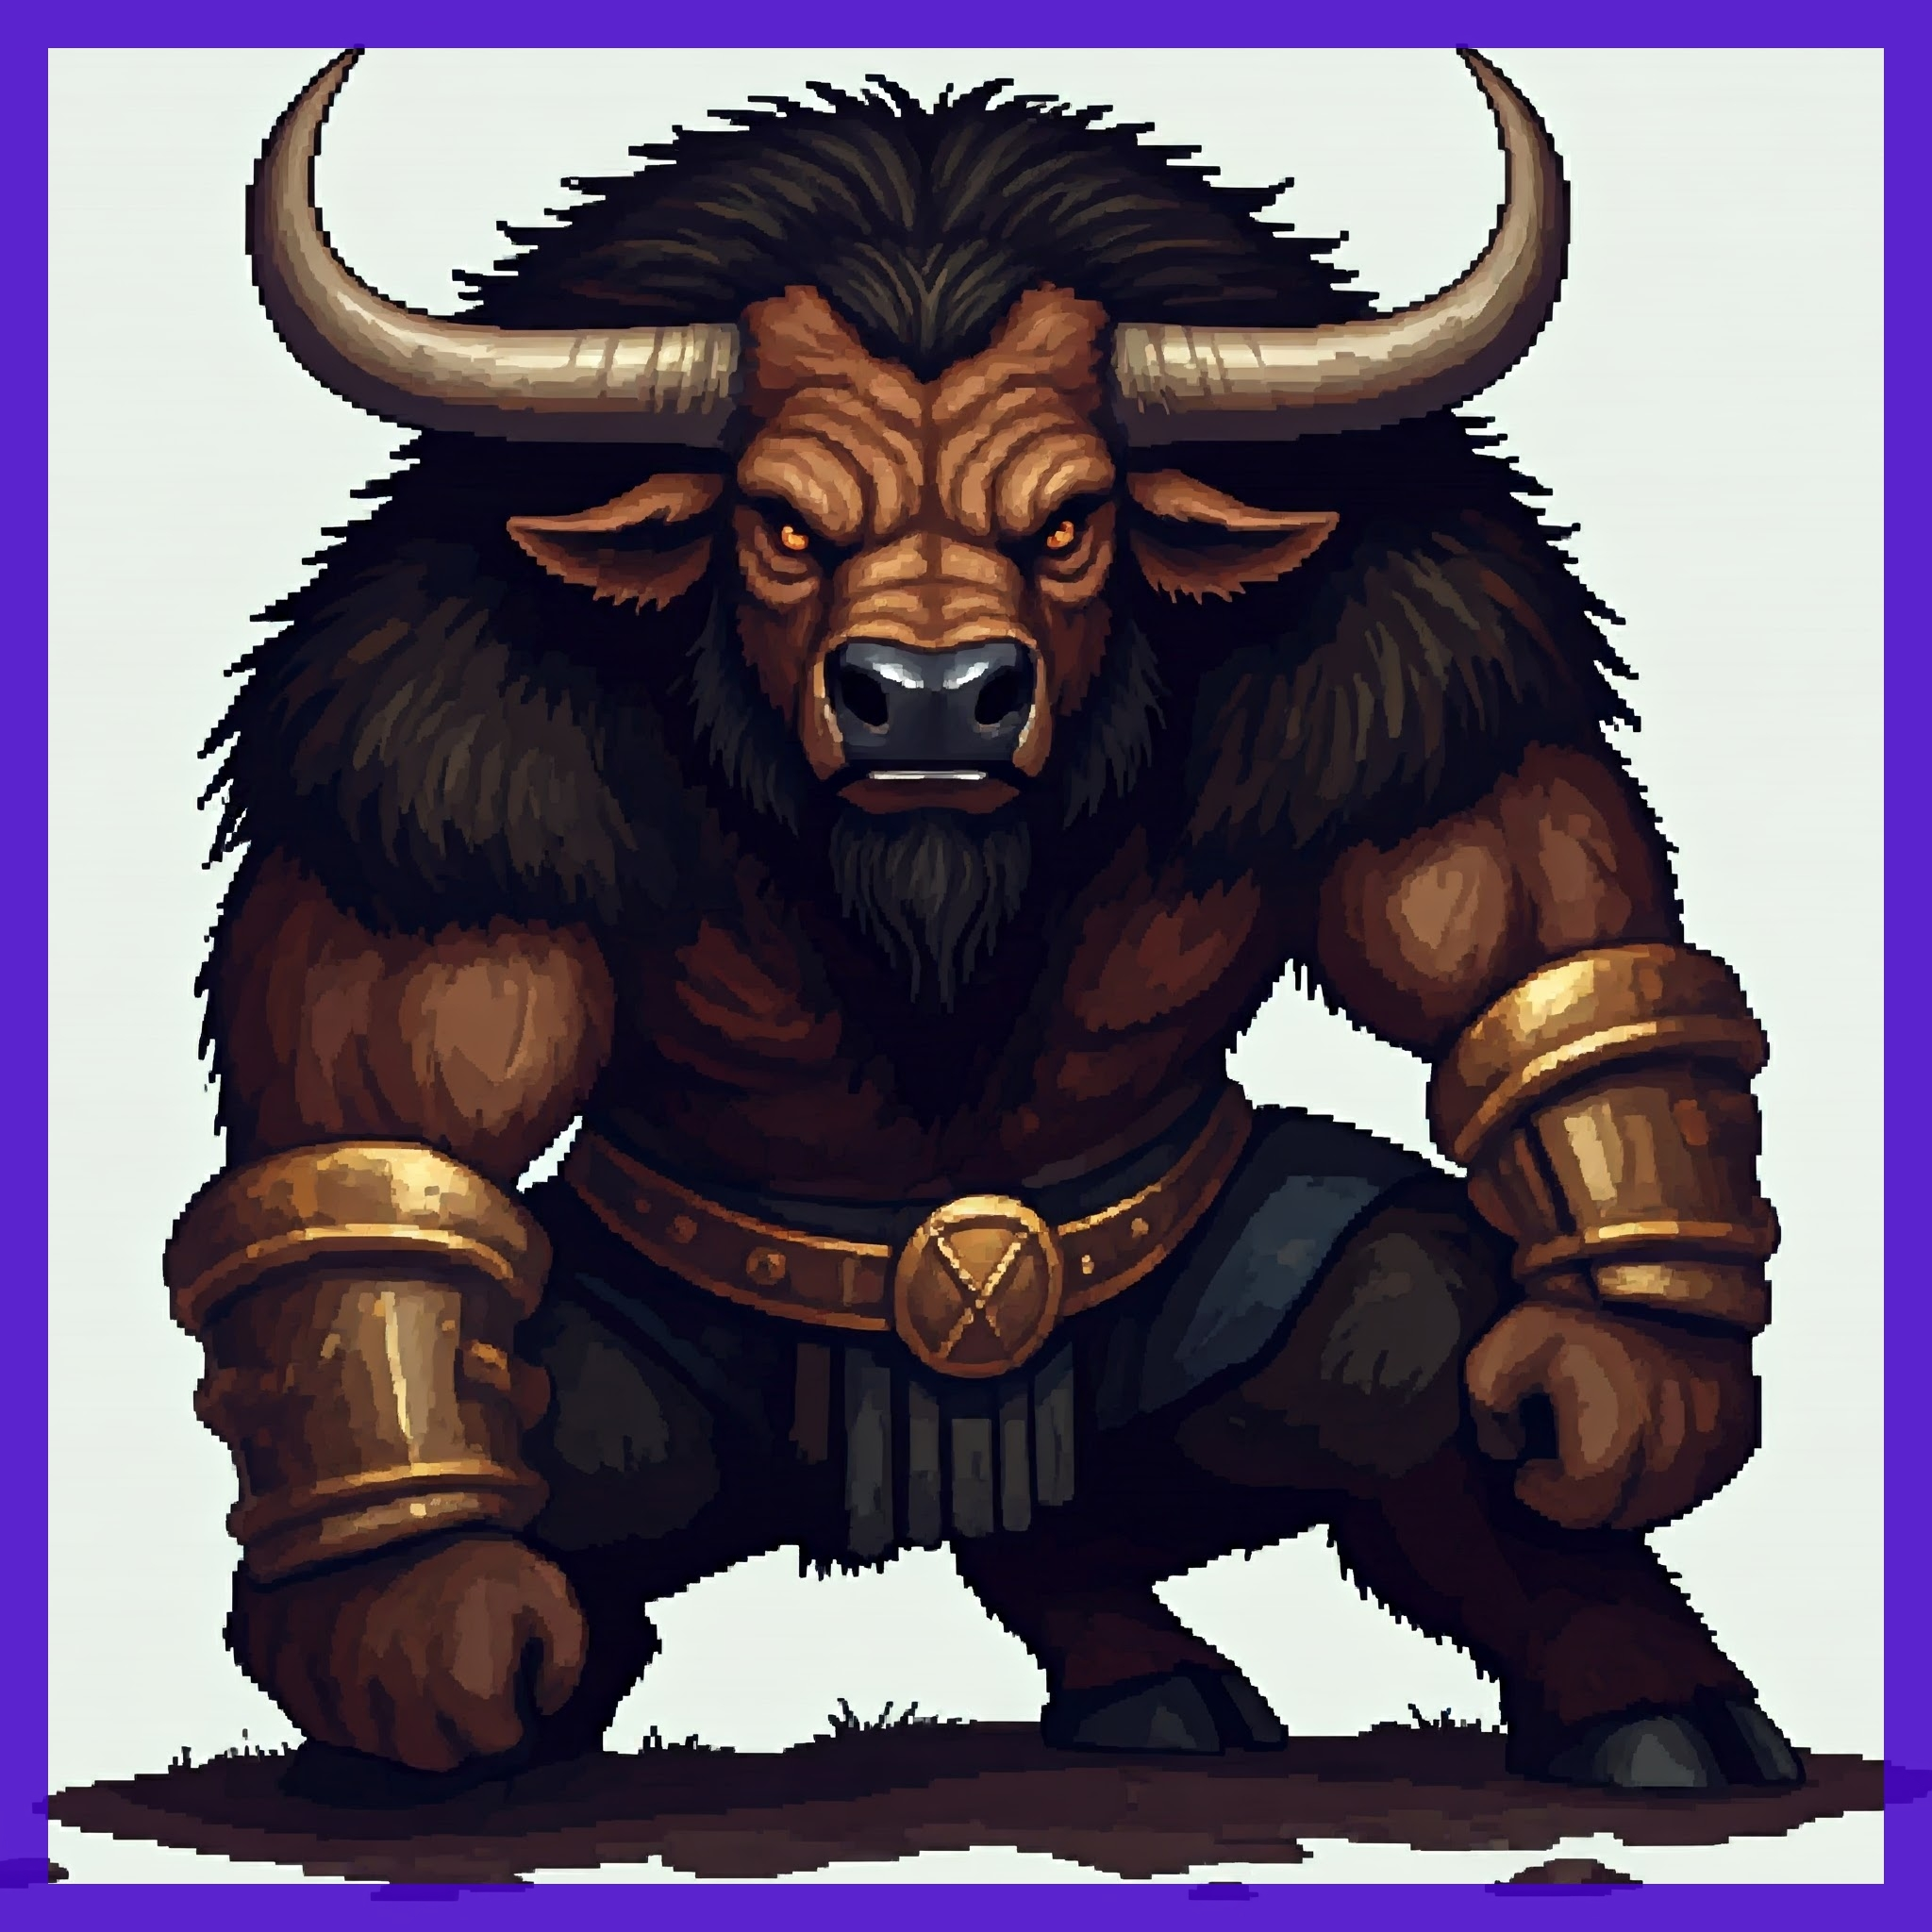
\includegraphics[width=.16\textwidth]{Minotaur (epic).jpg} & 
                    
\includegraphics[width=.16\textwidth]{Kraken (legendary).jpg} \\
                    
                    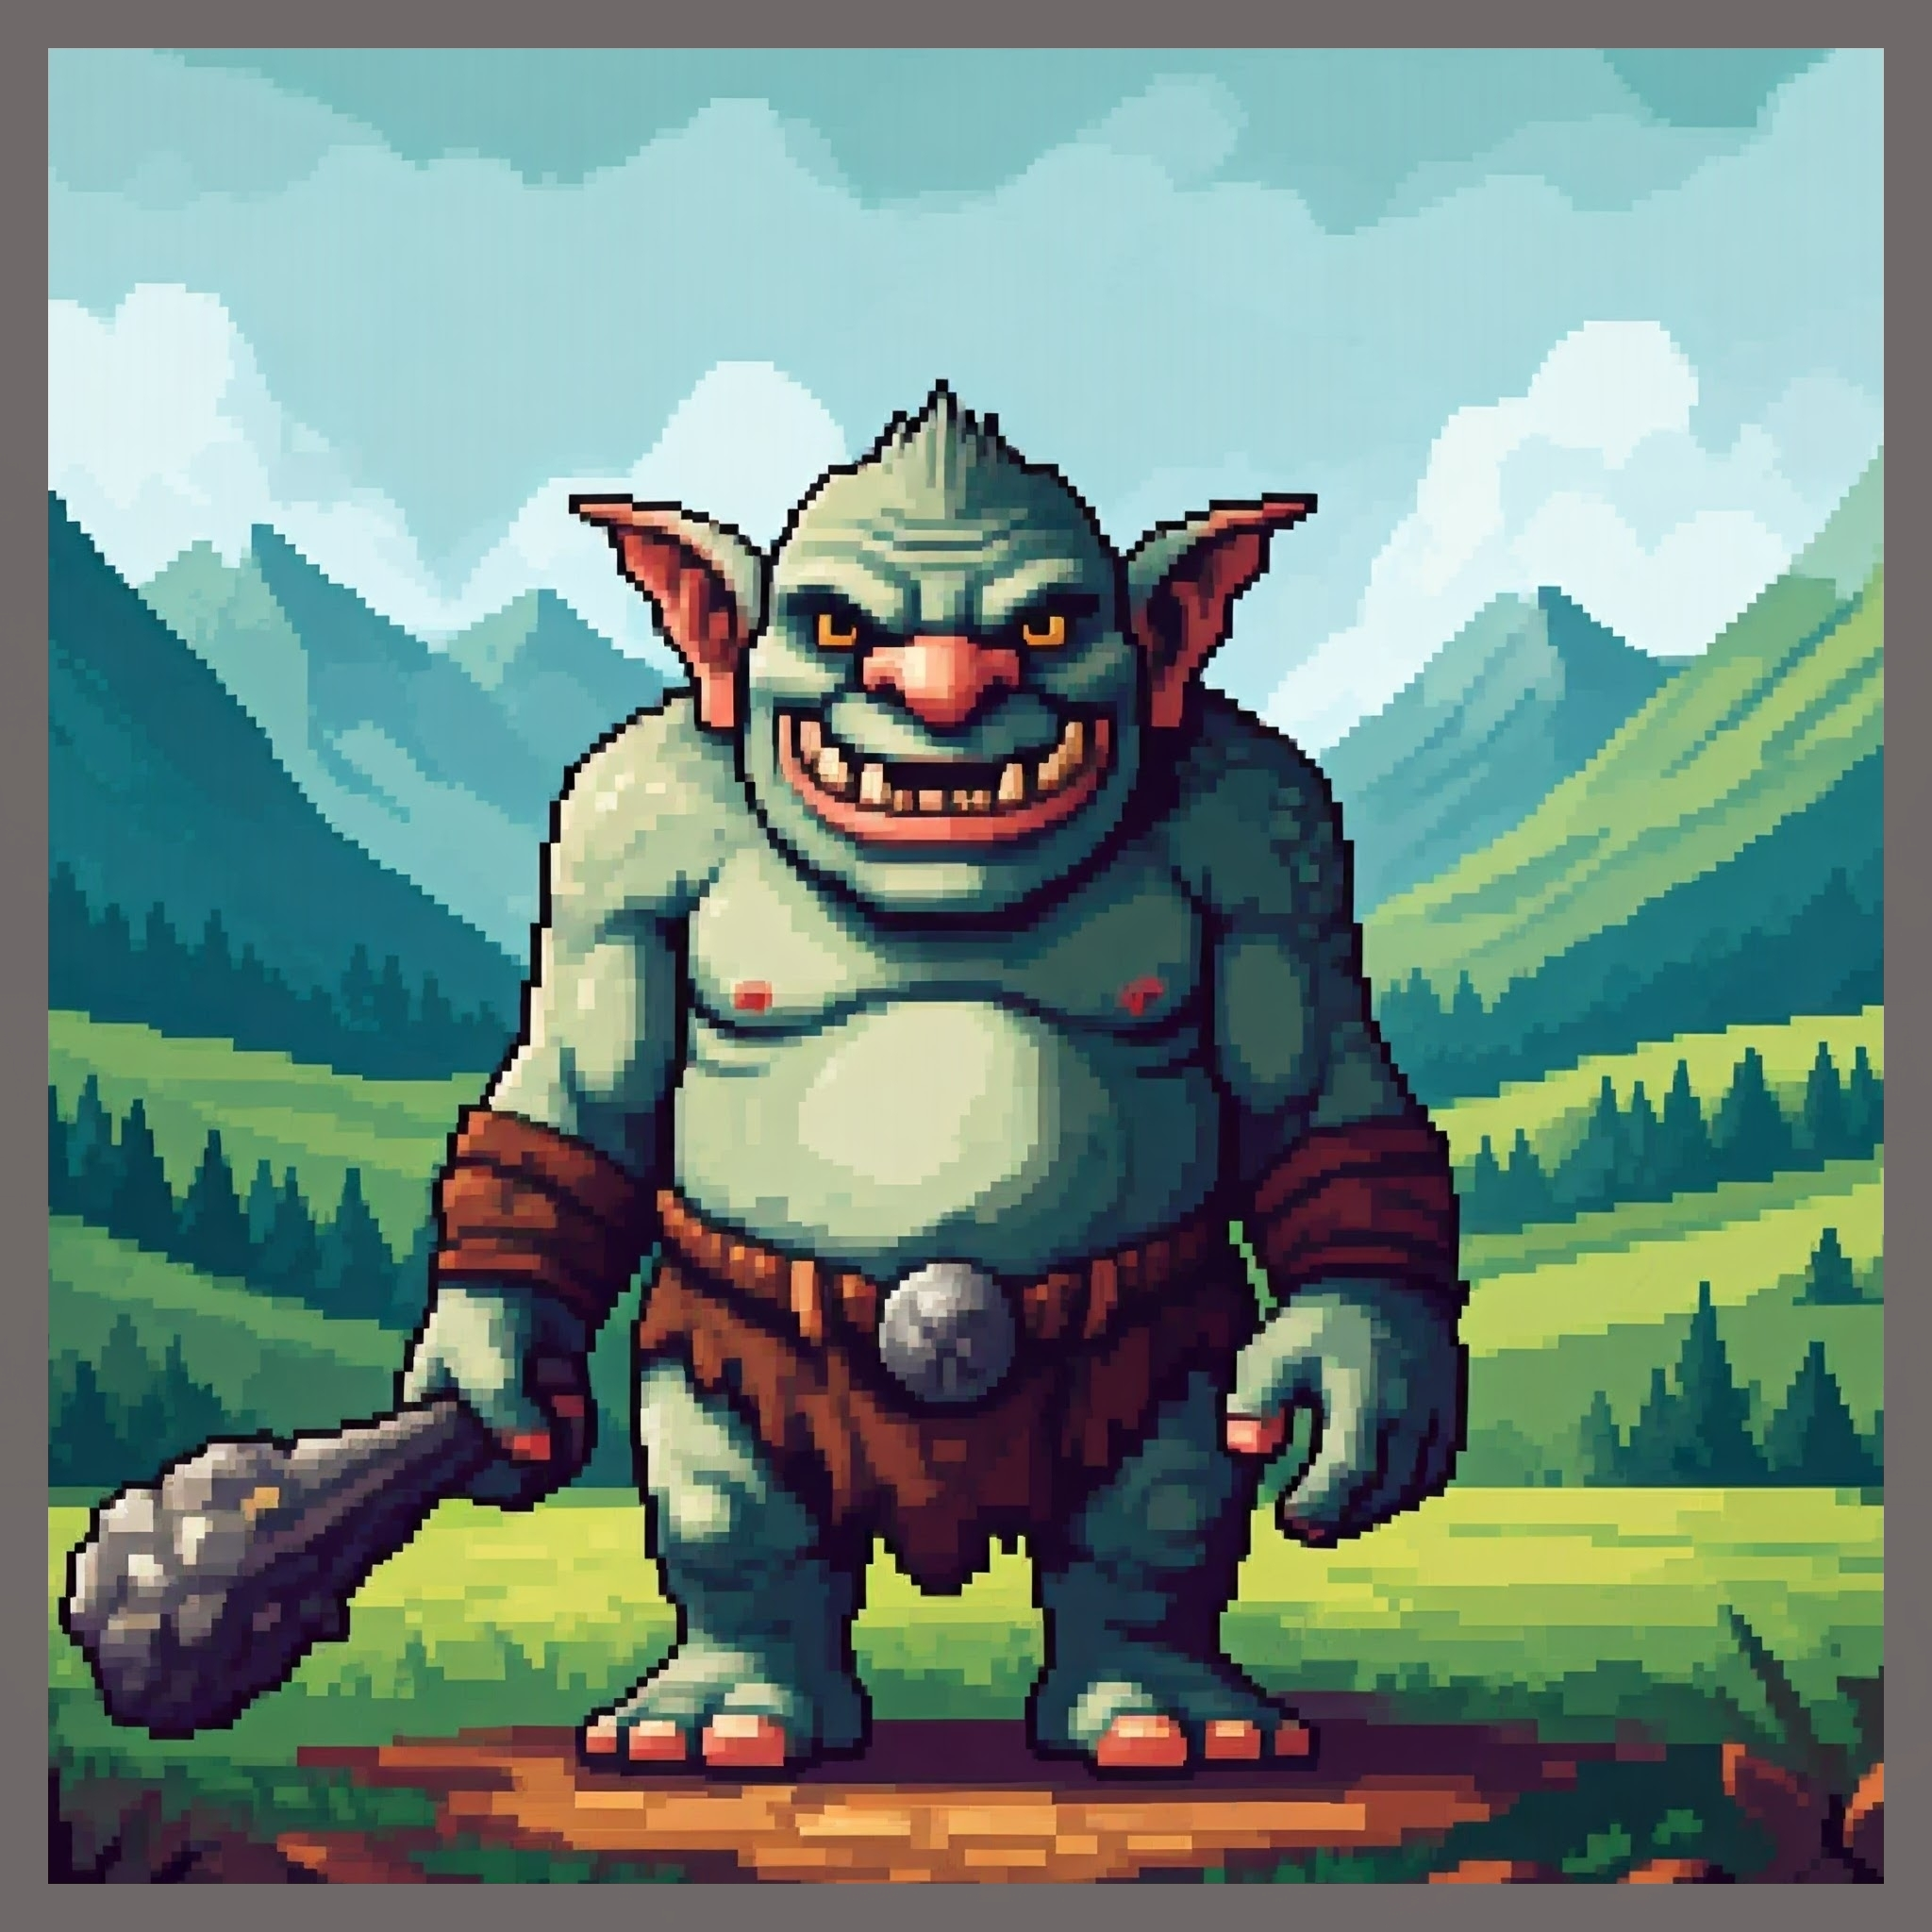
\includegraphics[width=.16\textwidth]{Orc (common).jpg} &
                    
\includegraphics[width=.16\textwidth]{Harpy (non-common).jpg} &
                    
\includegraphics[width=.16\textwidth]{Skeleton (rare).jpg} &
                    
\includegraphics[width=.16\textwidth]{Vampire (epic).jpg} & 
                    
\includegraphics[width=.16\textwidth]{Griffin (legendary).jpg} \\
                \end{tabular}
        \end{column}
        
        \begin{column}{.15\textwidth}
            \begin{tabular}{c}
                Currency \\[0.5ex]
                
\includegraphics[width=.90\textwidth]{Currency .png} \\[0.5ex]
                {\tiny \emph{Common} (C)} \\
                {\tiny \emph{Uncommon} (UC)} \\
                {\tiny \emph{Rare} (R)} \\
                {\tiny \emph{Epic} (E)} \\
                {\tiny \emph{Legendary} (S)}
            \end{tabular}
        \end{column}
    \end{columns}
\end{frame}

\begin{frame}{Architecture}
    \begin{center}
        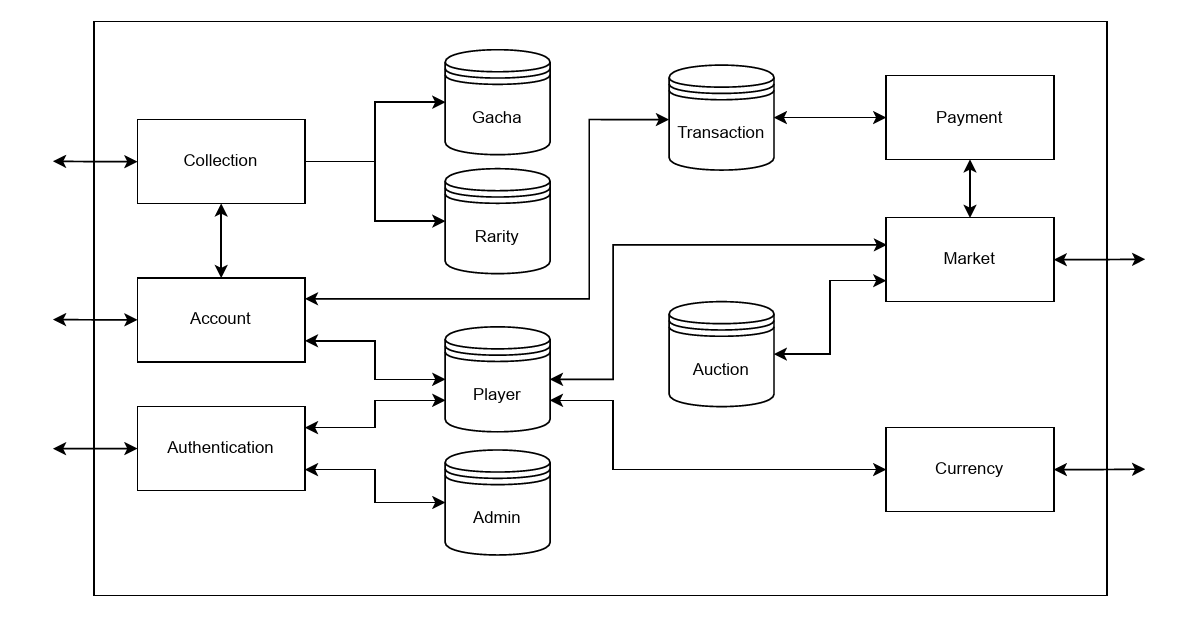
\includegraphics[scale=.65]{architecture-v1.png}
    \end{center}
\end{frame}

\begin{frame}{Architecture - details}
    The \textbf{authentication} component allows to log-in and log-out players and admins. \\[1ex]
    Using \textbf{account}, a player can check his own gacha collection and the transactions history. In particular, a transaction record is created only when an auction is completed (gacha rolls and currency purchasing are not considered as transactions). \\[1ex]
    The \textbf{market} component allows to discover active auctions and make bids, whereas \textbf{currency} component is used to purchase in-game currency. \\[1ex]
    The system gacha collection can be explored through \textbf{collection} component, which allows also to roll new gachas.
\end{frame}

\begin{frame}{Database}
    The gacha app is based on a single relational database which contains all the data inside different tables. In particular, we defined 6 main tables, i.e. \textbf{Player}, \textbf{Gacha}, \textbf{Auction}, \textbf{Transaction}, \textbf{Rarity} and \textbf{Admin}. Related to them, there are 2 \emph{join tables}, i.e. \textbf{Player\_Gacha} and \textbf{Player\_Auction}, which allow to maintain the user's gacha collection and user's bids. \\[1ex]
    An admin can only manage the application and \textbf{cannot} collect/buy gachas. \\[1ex]
    In the next slide we introduce the ER diagram and a brief description of it.  
\end{frame}

\begin{frame}{Database - ER diagram}
    \begin{center}
        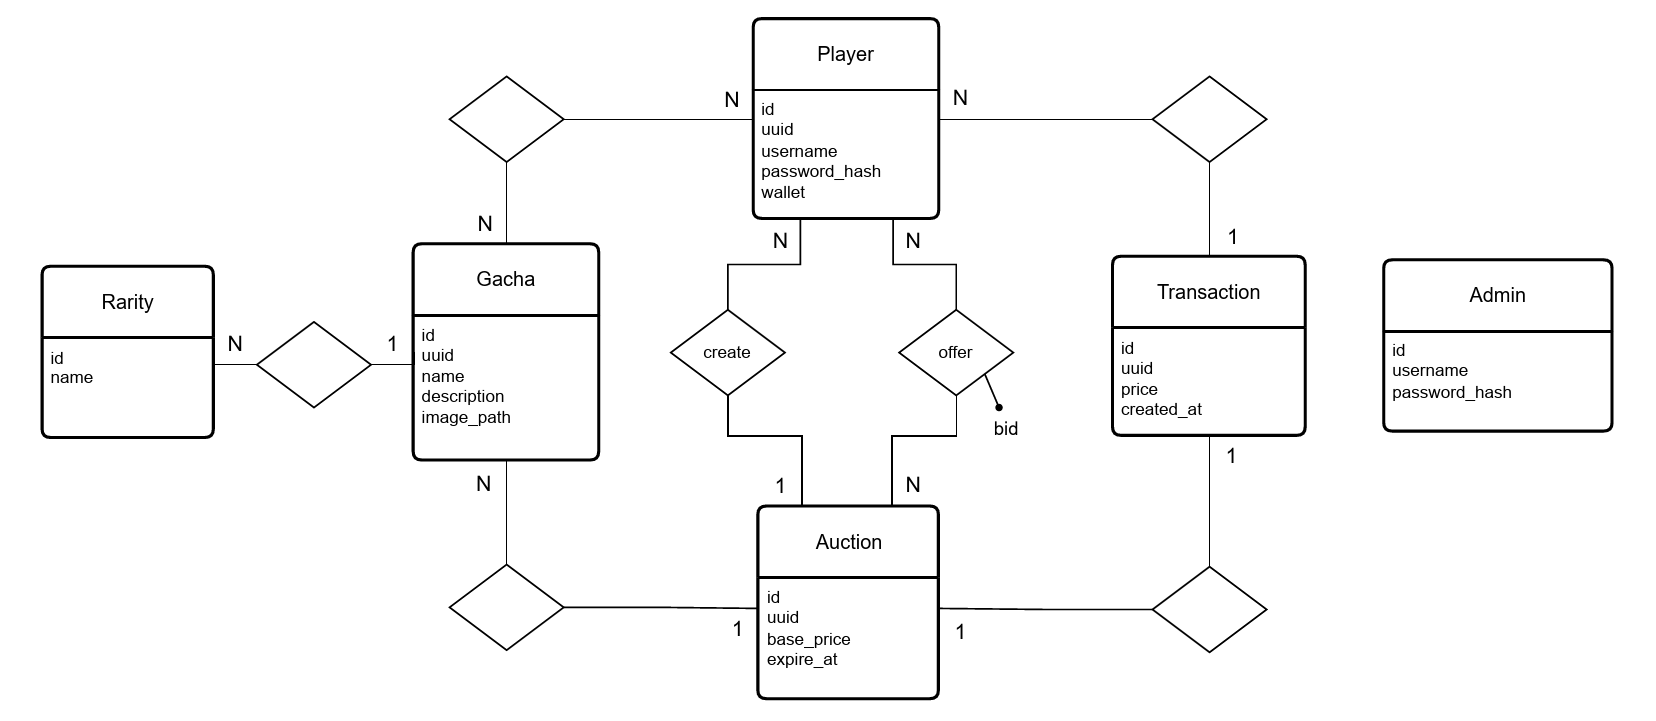
\includegraphics[scale=.5]{ASE-er-v4.png}
    \end{center}
\end{frame}

\begin{frame}{Database - ER diagram details}
    The \emph{N-to-N} relationship between \textbf{Player} and \textbf{Gacha} will be implemented with the table \textbf{Player\_Gacha}. The \textbf{Player\_Auction} table expresses the \emph{N-to-N} relationship between \textbf{Player} and \textbf{Auction}. When a player wins an auction and pays the gacha, a transaction record will be created. \\[1ex]
    Each auction is created by one player (i.e. \emph{create} relationship) and it will contain a reference to a transaction record when the winning player pays the bid. For \textbf{Transaction} records, we store the creation datetime. \\[1ex]
    The gacha's rarities are stored inside \textbf{Rarity} table and each gacha maintains a reference to a specific rarity.
\end{frame}

\begin{frame}{User's interactions}
      A player can do a bid only if he has enough currency. The payment operation will be done automatically by the system at the end of the auction. If he cannot pay (e.g. due to no found), the runner-up player will become the winner. \\[1ex]
     We consider in-coming transactions (i.e. player sells a gacha) and out-going ones (i.e. player buys a gacha). In the OpenAPI specifications, we use \textbf{from} and \textbf{to} attributes to distinguish between them.
\end{frame}

\end{document}
